\chapter{Detalles de Implementación y Experimentos}\label{chapter:implementation}

En este capítulo se toman decisiones claves respecto a qué herramientas utilizar para lidiar con problemas claves que surgen al autenticarse.

\section*{Elección de herramientas}
En la siguiente propuesta se utiliza LDAP como herramienta para ingerir datos. Como ya se ha explicado anteriormente, LDAP es el programa que se utiliza actualmente para unificar las distintas bases de datos de usuarios de toda la Universidad de La Habana. Para el manejo de LDAP se utilizará \textit{Apache Directory Studio} (ApacheDS), un software libre que permite la gestión de directorios.

También se utilizará Keycloak, una solución de gestión de acceso e identidad de código abierto dirigida a aplicaciones y servicios modernos. Esta facilita la protección de aplicaciones y servicios con poco o ningún código [\cite{muyon2020metodos}]. 

Esta es una herramienta que se encarga de abstraer la parte de autenticación de usuarios y almacenamiento de información privada de estos, del flujo de comunicación entre cliente y servidor. Ofrece \textit{Single Sign-On} a través de una autenticación basada en tokens y está diseñada para que sea sencillo añadir nuevos servidores de usuarios y clientes.

Keycloak contiene una alta elegibilidad de configuración en sí mismo. Su papel es meramente intermediario entre servicios externos, por lo que cuando un usuario quiere iniciar sesión en una aplicación, la autenticación se le transfiere directamente al servicio Keycloak, que se encarga de generar los objetos JWT que se envían necesariamente entre servicios para transmitir los datos de dicho usuario.

Este servicio ofrece un amplio abanico de posibilidades en la configuración del acceso entre servicios. Se ha elegido frente a otras soluciones de código abierto como STYTCH, Ory, Okta o Auth0 porque Keycloak ofrece un nivel más alto en cuanto a rendimiento, escalabilidad y disponibilidad [\cite{lobato2022regulacion}]. 

Gluu es otra de las tecnologías que tienen prestaciones y ventajas similares a Keycloak. Es un servicio \textit{Open Source} que soporta \textit{SAML}, \textit{OpenID Connect}, \textit{SSO} y \textit{OAuth 2.0}. Sin embargo \textit{Gluu} es un sistema que requiere de 8 GB de RAM y 40 GB de espacio en disco, mientras que Keycloak solo necesita de 512 Mb de RAM y 1 GB de disco. Por ello la segunda tecnología se ajusta más a los recursos con que cuenta  la Universidad de La Habana [\cite{vassallo2017continuous}].

Para la experimentación se creará un cliente capaz de interactuar con el sistema implementado para autenticar usuarios. Keycloak permite proteger aplicaciones que se ejecutan en diversas plataformas y tecnologías que usan los protocolos \textit{OpenID Connect } y SAML [\cite{secure_apps_2022}]. 

Entre los soportes ofrecidos, se ha escogido la biblioteca de Python \href{https://pypi.org/project/python-keycloak/}{\textcolor{blue}{\textbf{Python Keycloak}}}, que provee fácil acceso a la API de Keycloak. Python es un lenguaje de programación que permite trabajar rápido e integrar sistemas eficientemente [\cite{python_2022}]. Podría decirse que durante la última década Python se ha convertido en uno de los lenguajes de código abierto más utilizados.

Para la visualización de la solución se utiliza Flask, un \textit{micro framework} de Python que proporciona las funcionalidades básicas de\textit{ web frameworks}.

\section*{Ingestión de Datos}

\subsection*{Herramientas para el uso de LDAP}

A partir del protocolo LDAP se han desarrollado diversas implementaciones por parte de algunas empresas o fundaciones. El cuadro siguiente lista algunas de las implementaciones de este protocolo, así como la empresa o fundación detrás de esta y el tipo de licencia con que es distribuido [\cite{gonzalez2010implementacion}]:

\begin{table}[H]
	\centering
	\begin{tabular}{ |p{4cm}|p{4cm}|p{4cm}| }
		\hline
		\textbf{Software}&\textbf{Empresa que lo desarrolla}&\textbf{Tipo de licencia}\\
		\hline
		Novell eDirectory  &  Novell, Inc.  & Privativa\\
		\hline
		Red Hat Directory Server& Red Hat, Inc.&Libre (GPL)\\
		\hline
		Active Directory &Microsoft Corporation& Privativa\\
		\hline
		Open Directory &Apple Inc.& Privativa\\
		\hline
		Apache Directory Serve&   Apache Software Foundation& Libre (Apache License)\\
		\hline
		Oracle Internet Directory&Oracle Corporation& Privativa\\
		\hline
		OpenDS&Sun Microsystems & Libre (CDDL)\\
		\hline
		OpenLDAP&OpenLDAP Foundation& Libre (OpenLDAP Public License)\\
		\hline
		IBM Tivoli Directory Server&IBM& Privativa\\
		\hline
	\end{tabular}
	\caption{\label{tab:table-name}Diferentes implementaciones del protocolo LDAP.}
\end{table}

Teniendo en cuenta la tabla previa, se puede extraer una serie de opciones candidatas de servicios de directorios que tienen la posibilidad de ser implementados, tomando como base solo dos criterios de elección seleccionados: que sea software libre y que sea gratuito. Realizando la clasificación bajo estos
lineamientos, las opciones elegibles son:

\begin{itemize}
	\item \textit{Apache Directory Server}
	\item \textit{OpenDS}
	\item \textit{OpenLDAP}
\end{itemize}

Además, se comprobó un tercer criterio al realizar las pruebas a las opciones candidatas, el cual fue la capacidad de despliegue de dicha solución en diferentes sistemas operativos. \textit{OpenLDAP} no se ecuentra disponible en el sitio oficial para Windows, sistema operativo utilizado en el Node Central, por lo cual no se utilizará. 

\textit{ApacheDS} tiene una documentación amplia y es fácil de desplegar. También cuenta con instaladores fáciles de usar para diversos sistemas operativos, entre los cuales se encuentran Linux, Solaris, Mac OS X y Windows. Además provee el código fuente en caso que sea necesaria su compilación. Por lo tanto, esta será la herramienta utilizada para acceder a LDAP.

\textit{ApacheDS} cuenta con una herramienta bastante completa para la gestión del directorio llamada \textit{Apache Directory Studio} la cual está basada en el entorno de desarrollo Eclipse. Esta se utilizará para acceder a los dos LDAP con los que se interactúa, la de los trabajadores y la de los estudiantes.

\subsection*{Keycloak como herramienta para la ingestión de datos}
%
%Cómo se instala LDAP?
%Cómo se configura Keycloak con dos LDAPs?

Para la instalación y configuración de Keycloak se siguen las guías: \href{https://www.keycloak.org/getting-started/getting-started-zip}{\textcolor{blue}{\textit{Keycloak Get Started}}} y \href{https://www.keycloak.org/server/configuration}{\textit{\textcolor{blue}{Configuring Keycloak}}}. En esta solución se utiliza \href{https://github.com/keycloak/keycloak/releases/download/20.0.1/keycloak-20.0.1.zip}{\textcolor{blue}{keycloak-20.0.1.zip}}.

Se realizan las siguientes configuraciones:


\begin{enumerate}
	\item \textbf{Creación de usuario administrador}
	
	Para ello se debe abrir \href{http://localhost:8080/}{\textcolor{blue}{http://localhost:8080/}}
	y rellenar el formulario con el nombre de usuario y contraseña de preferencia.
	
	\begin{figure}[H]
		\centering
		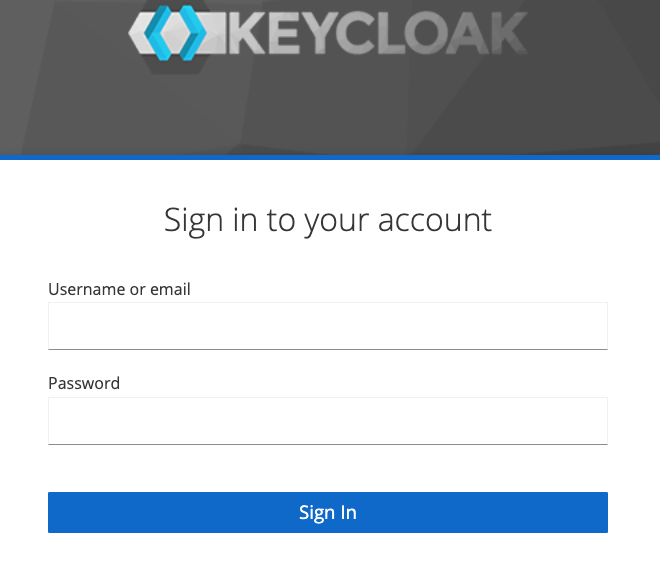
\includegraphics[width=0.7\linewidth]{Graphics/admin_console}
		\caption{Usuario Administrador}
		\label{fig:adminconsole}
	\end{figure}
	
	
	\item \textbf{Creación de \textit{REALM}}
	
	Keycloak crea \textit{Realms} o reinados separados y no accesibles entre ellos y administra clientes, usuarios y otras entidades dentro de estos. Cada \textit{realm} tiene su propia configuración.
	\begin{figure}[H]
		\centering
		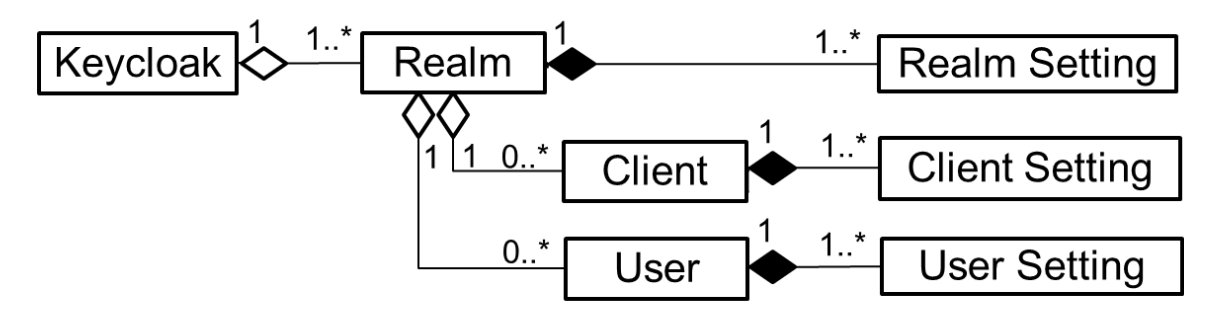
\includegraphics[width=0.9\linewidth]{Graphics/keycloak_realm}
		\caption{Relación de entidades en Keycloak}
		\label{fig:keycloakrealm}
	\end{figure}
	En este caso se necesita un único sistema para la autenticación de varios clientes, por lo que solo se utilizará un \textit{realm} llamado \textit{Master}.
	
	\item \textbf{Creación de \textit{User Federation}}
	
	Keycloak puede almacenar y administrar usuarios. A menudo las instituciones ya tienen los servicios de LDAP o \textit{Active Directory} para guardar los usuarios y las credenciales. Keycloak es capaz de validar credenciales y extraer información de fuentes externas. [\cite{keycloak_2022}]
	
	\begin{figure}[H]
		\centering
		\includegraphics[width=1\linewidth]{"Graphics/keycloak_user federation"}
		\caption{Keycloak: \textit{User Federation}}
		\label{fig:keycloakuser-federation}
	\end{figure}
	
	
	En este caso, la información se extraerá de LDAP. Por lo tanto, la configuración será la siguiente:
	
	\begin{figure}[H]
		\centering
		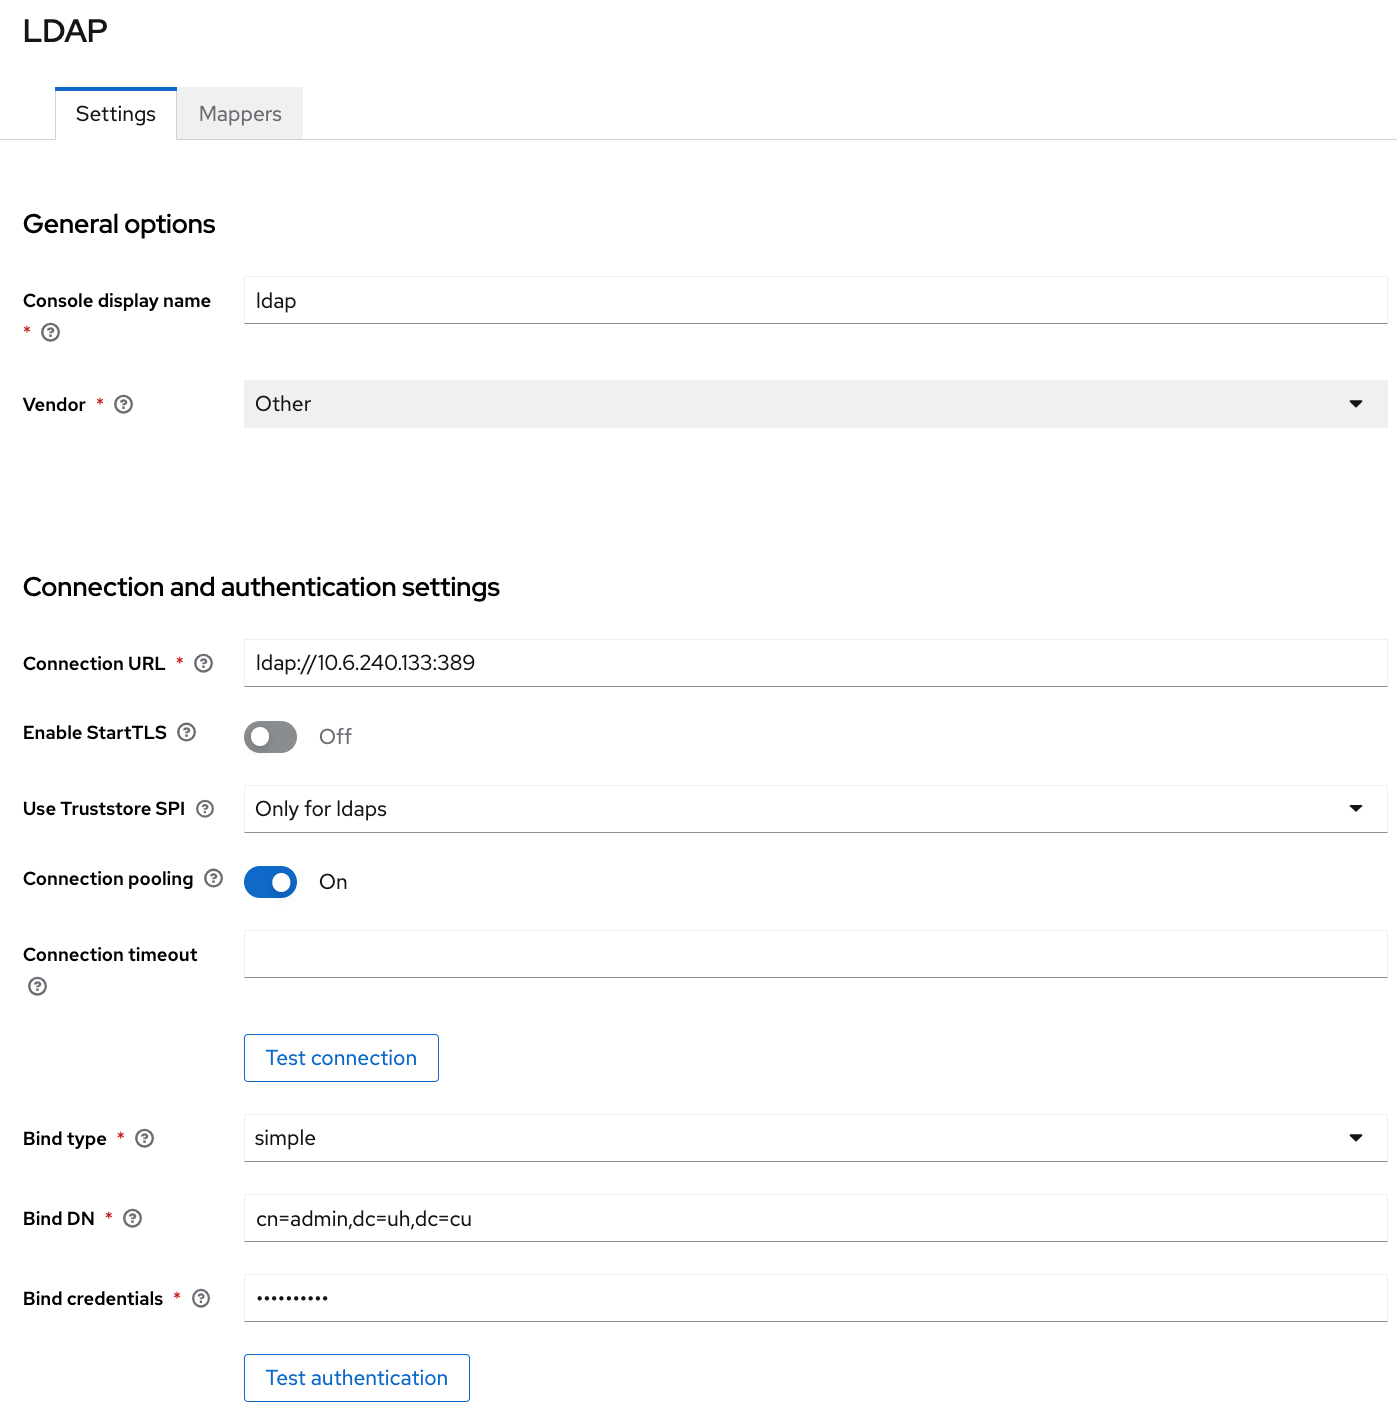
\includegraphics[width=0.9\linewidth]{Graphics/keycloak_configuracion_ldap1}
		\caption{Configuración de LDAP en Keycloak}
		\label{fig:keycloakconfiguracionldap1}
	\end{figure}
	
		\begin{figure}[H]
		\centering
		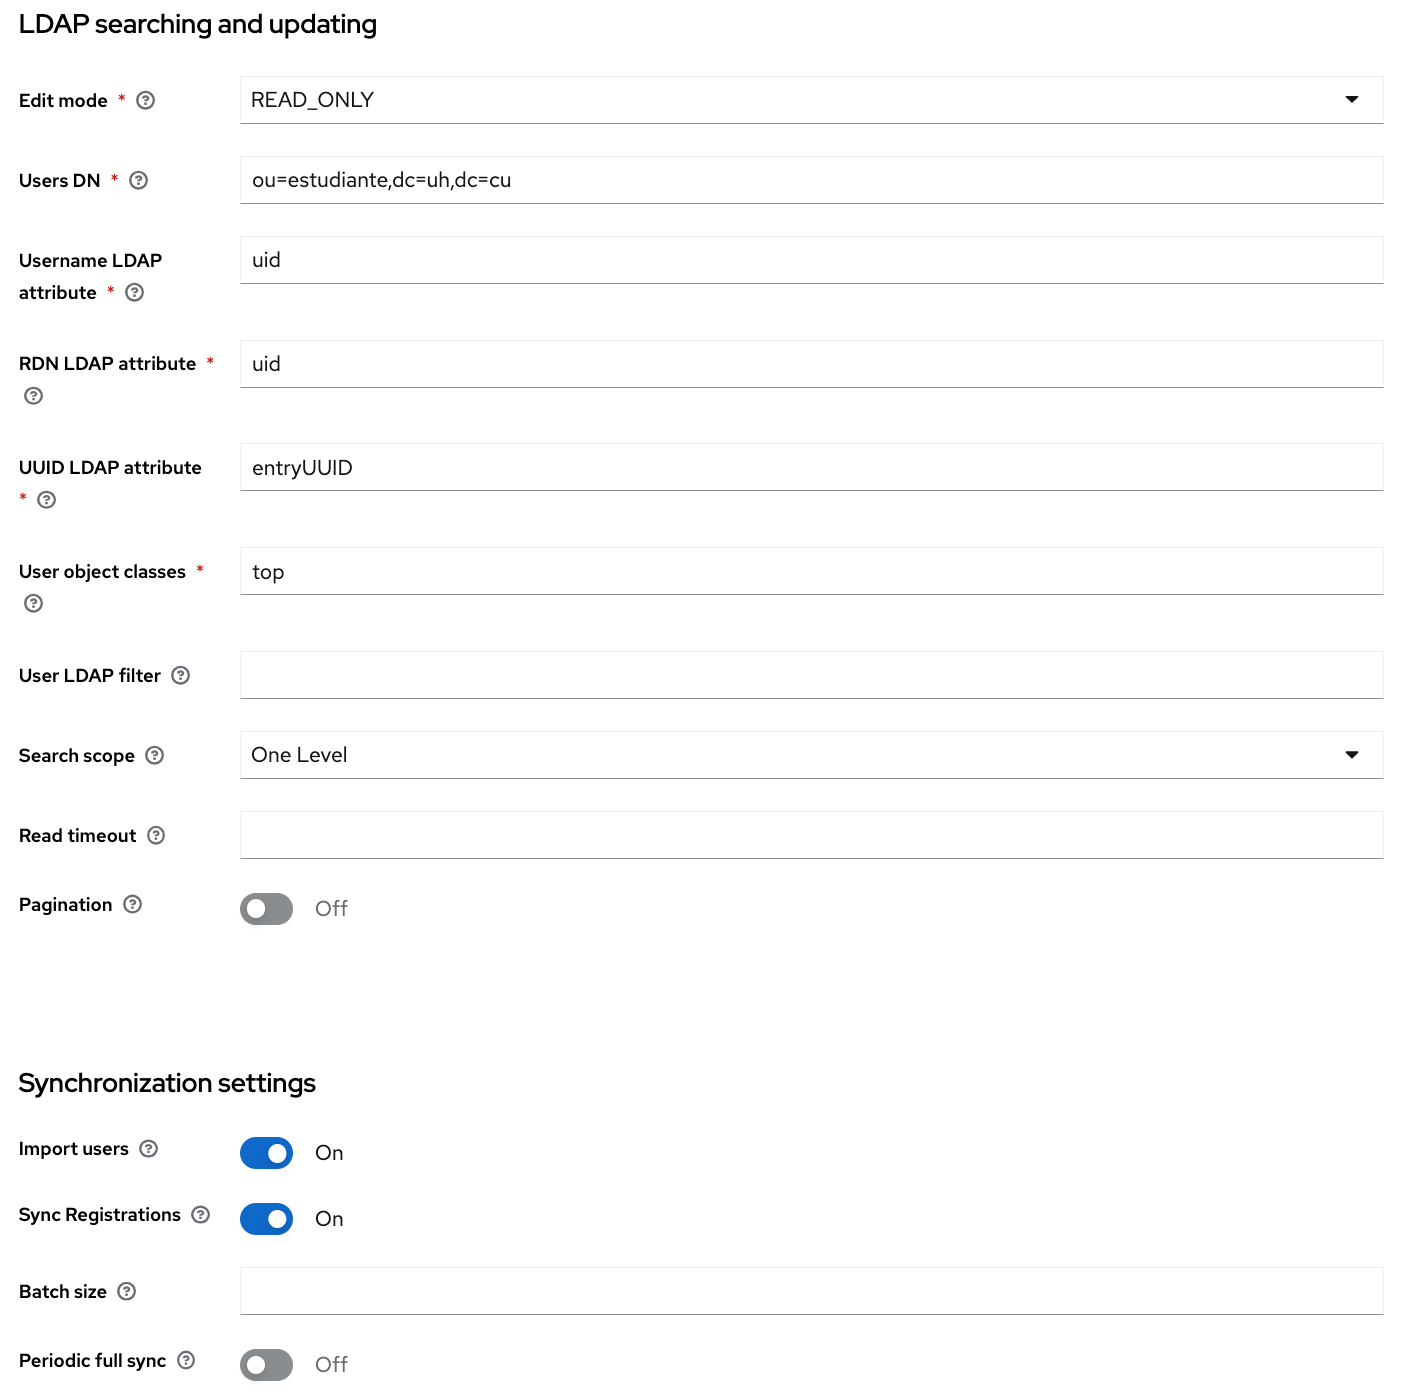
\includegraphics[width=0.9\linewidth]{Graphics/keycloak_configuracion_ldap2}
		\caption{Configuración de LDAP en Keycloak}
		\label{fig:keycloakconfiguracionldap1}
	\end{figure}

	Luego de conectar Keycloak con LDAP, se puede comprobar que los usuarios sincronizan. En la siguiente imagen se pueden ver los usuarios en LDAP desde \textit{Apache Directory Studio}:
	
	\begin{figure}[H]
		\centering
		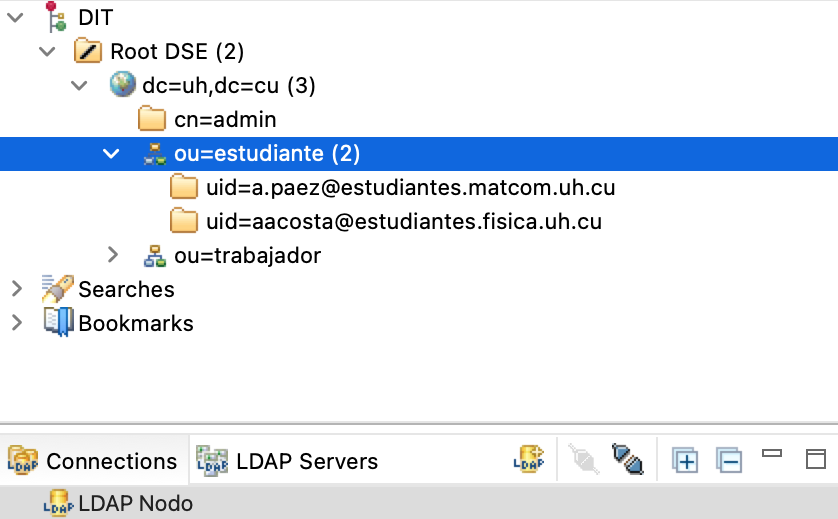
\includegraphics[width=0.7\linewidth]{Graphics/ADS_usuarios}
		\caption{Usuarios en LDAP vistos desde \textit{Apache Directory Studio}}
		\label{fig:adsusuarios}
	\end{figure}

	En la siguiente imagen se puede comprobar que Keycloak sincroniza todos los usuarios de LDAP:
	
		\textcolor{red}{*Insertar imagen*}

\end{enumerate}





 

Cómo se configuran los permisos por grupo de usuarios?

\section*{Capa de autenticación}


Para la autenticación se necesita un nombre de usuario único para cada trabajador y estudiante de la institución. Al utilizarse distintas fuentes de datos, no se puede garantizar que todas las bases de datos tengan las mismas estructuras. Sin embargo, todos los usuarios tienen una cuenta de correo que los identifica unívocamente, por lo que utilizar este campo como nombre de usuario garantiza que cada persona es identificada.

En el siguiente diagrama se muestra el flujo de información que se realiza para el correcto funcionamiento de la autenticación:

\begin{figure}[H]
	\centering	
	\hspace*{-0.3in}
	\includegraphics[width=1.1\linewidth]{"Graphics/diagrama de flujo del prototipo del servicio"}
	\caption{Diagrama de flujo de información}
	\label{fig:diagrama-de-flujo-del-prototipo-del-servicio}
\end{figure}

Cada paso descrito en el diagrama de flujo se explica detalladamente a continuación: 

\begin{itemize}
	\item La primera acción (1) consiste en que el cliente haga login en el sistema por medio de unas credenciales básicas que son su identificador y contraseña. Esta petición se redirigirá automáticamente al servidor Keycloak, el único que contiene la información almacenada de los clientes del sistema, así como sus credenciales. 
	
	\item El segundo paso (2), viene con la validación de dichas credenciales en la aplicación de autenticación Keycloak, y la generación de un \textit{Access Token}.
	
	\item El tercer paso (3) es el envío de dicho token a través de JWT hacia el usuario o aplicación cliente. Sin embargo, en caso de que las credenciales hayan resultado erróneas, se enviará el mensaje de error correspondiente. 
	
	\item En el cuarto paso (4), la aplicación cliente ya iniciada sesión, dispone del \textit{Access Token} para realizar consultas, por lo que genera la primera petición de algún recurso cualquiera al servidor del Nodo.
	
	\item El paso denominado X es la validación instantánea del token que contiene la petición del cliente. Antes de entrar en la lógica de interfaz que ofrece la API del servidor, cabe mencionar aquí que se ha insertado un denominado “Interceptor”. Este, procesa el JWT que le llega en la petición al servidor y valida toda la información del mismo. Este paso se repite por lo tanto en varias ocasiones, para cada petición de recurso ya que cada recurso requiere unos permisos o scopes específicos. 
	
	\item El quinto (5) paso consiste en la generación de la respuesta que envía el servidor a la aplicación cliente en caso de validación de token correcta. 
	
	\item El sexto paso (6) esta vez corresponde a otra petición de recurso distinta, que será seguida de una errónea validación de token en el paso X.
	
	\item El séptimo paso (7) corresponde al envío del mensaje de error a la aplicación cliente, que será tratado como expiración del token, y le pedirá una extensión o actualización de la sesión. 
	
	\item El octavo paso (8) corresponde al consecuente envío del \textit{refresh token}, que sirve para extender la sesión actual. Es el mecanismo que se lleva a cabo a bajo nivel en cualquier sesión abierta de un servicio web.
	
	\item En el noveno paso (9) se produce una validación de este \textit{refresh token}, y la obtención de un nuevo \textit{Access Token} que se obtiene de forma similar pero no igual al mencionado en el segundo paso (2). 
	
	\item En el décimo paso (10) se envía este último token generado a la aplicación cliente de manera que este podrá realizar nuevas peticiones. 
	
	\item En los pasos undécimo (11) y duodécimo (12) el escenario se repite de forma
	iterativa hasta que el cliente decidiese acabar en el último paso: 
	
	\item El paso N consiste en el cierre de sesión por parte del cliente y por lo tanto la comunicación se cierra en este ciclo. 
	
\end{itemize}


\section*{Clientes}

\subsection*{Configuración de cliente Keycloak}

Keycloak permite añadir clientes de forma sencilla. En las siguientes imágenes se muestra paso a paso como se agrega un nuevo cliente al sistema:

\begin{figure}[H]
	\centering
	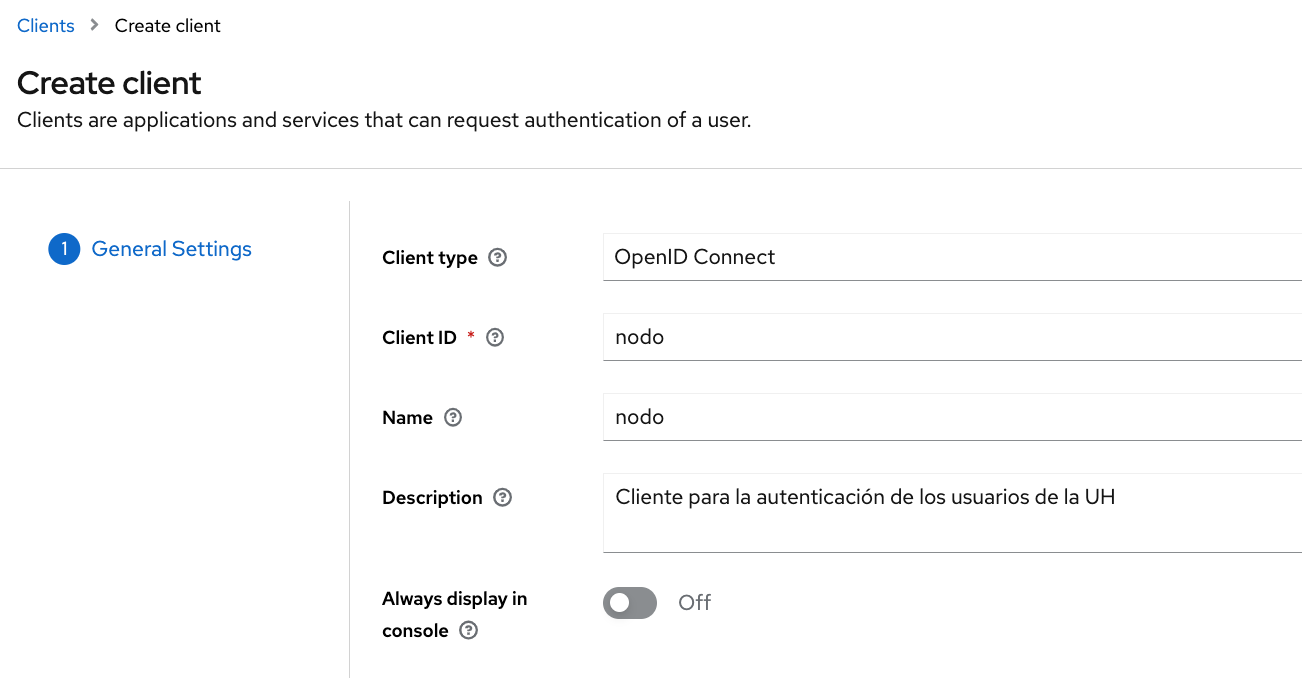
\includegraphics[width=1\linewidth]{Graphics/client_new1}
	\caption{Nuevo cliente en Keycloak}
	\label{fig:clientnew1}
\end{figure}

\begin{figure}[H]
	\centering
	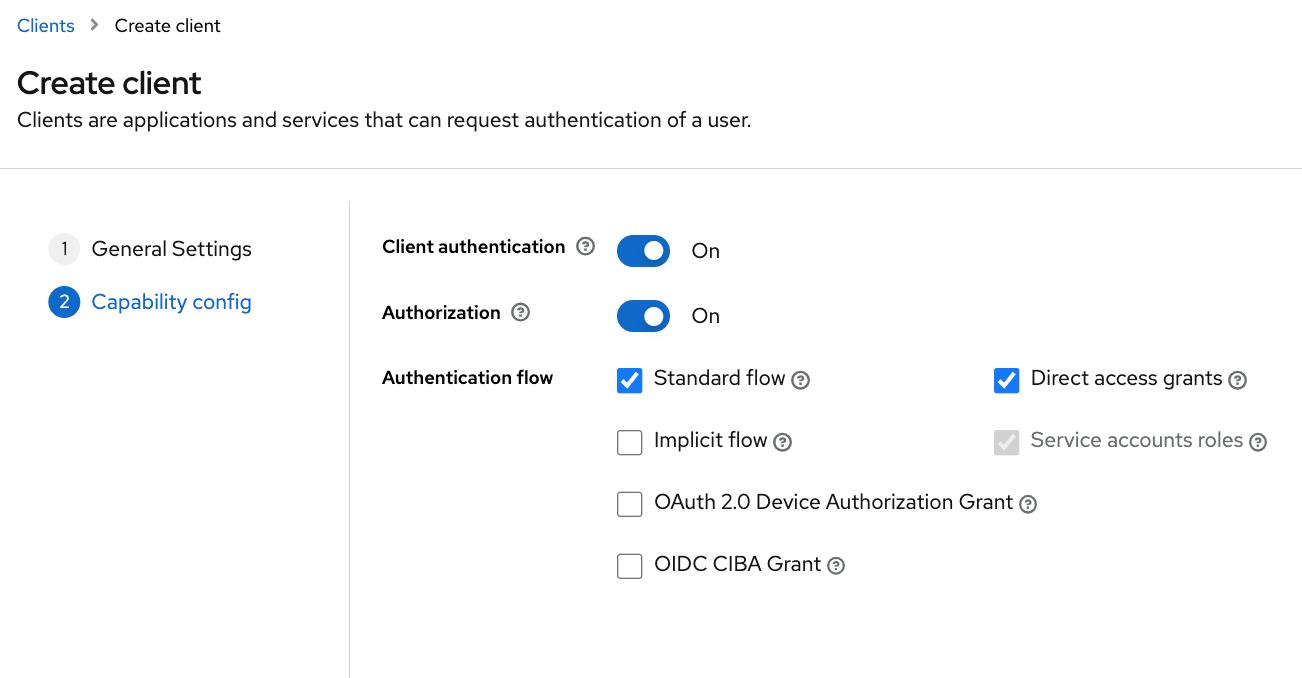
\includegraphics[width=1\linewidth]{Graphics/client_new2}
	\caption{Nuevo cliente en Keycloak}
	\label{fig:clientnew2}
\end{figure}

Luego se puede ver el nuevo cliente nodo en la lista de clientes:

\begin{figure}[H]
	\centering
	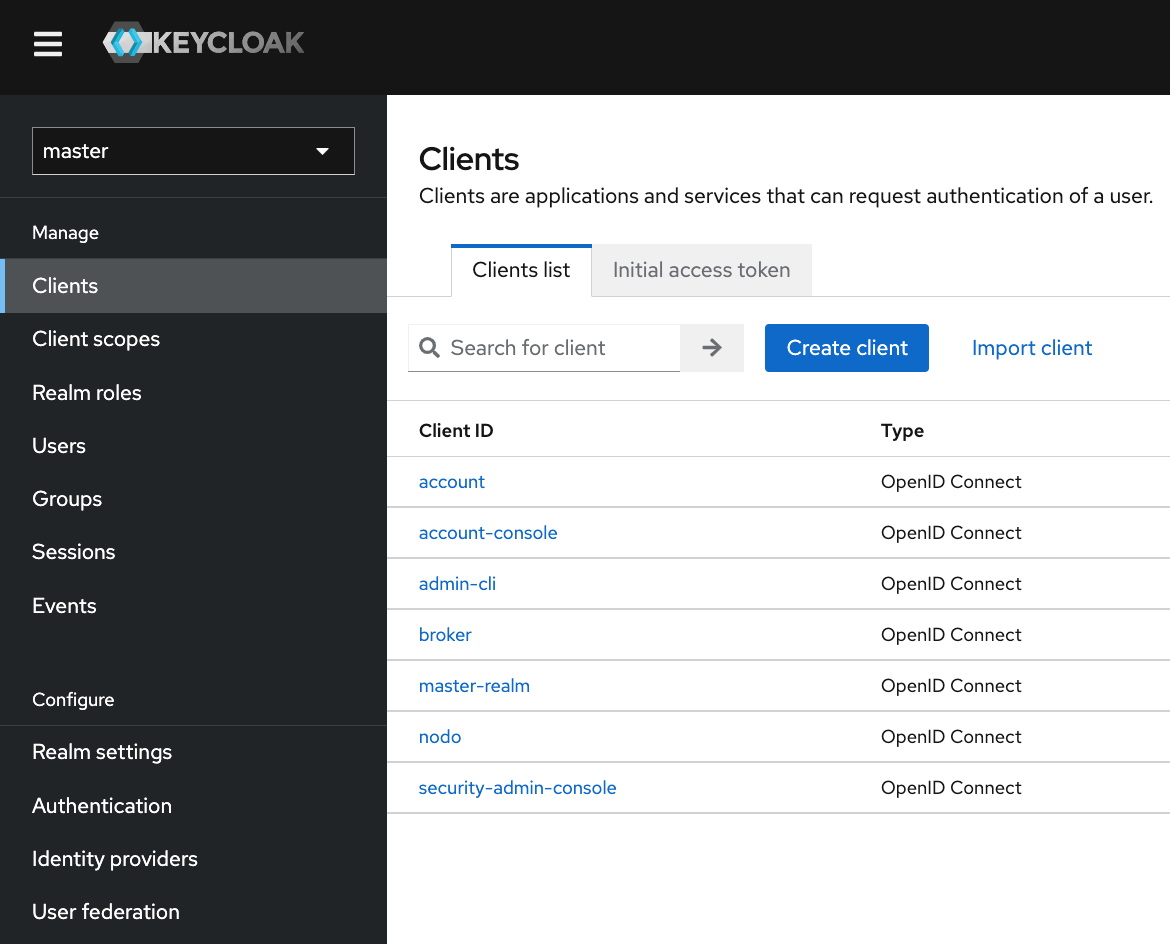
\includegraphics[width=0.9\linewidth]{Graphics/client_list}
	\caption{}
	\label{fig:clientlist}
\end{figure}

Luego de crear el cliente, se puede este conectar a los servicios de Keycloak con la correcta configuración. Para ello será necesario utilizar las credenciales del cliente:

\begin{figure}[H]
	\centering
	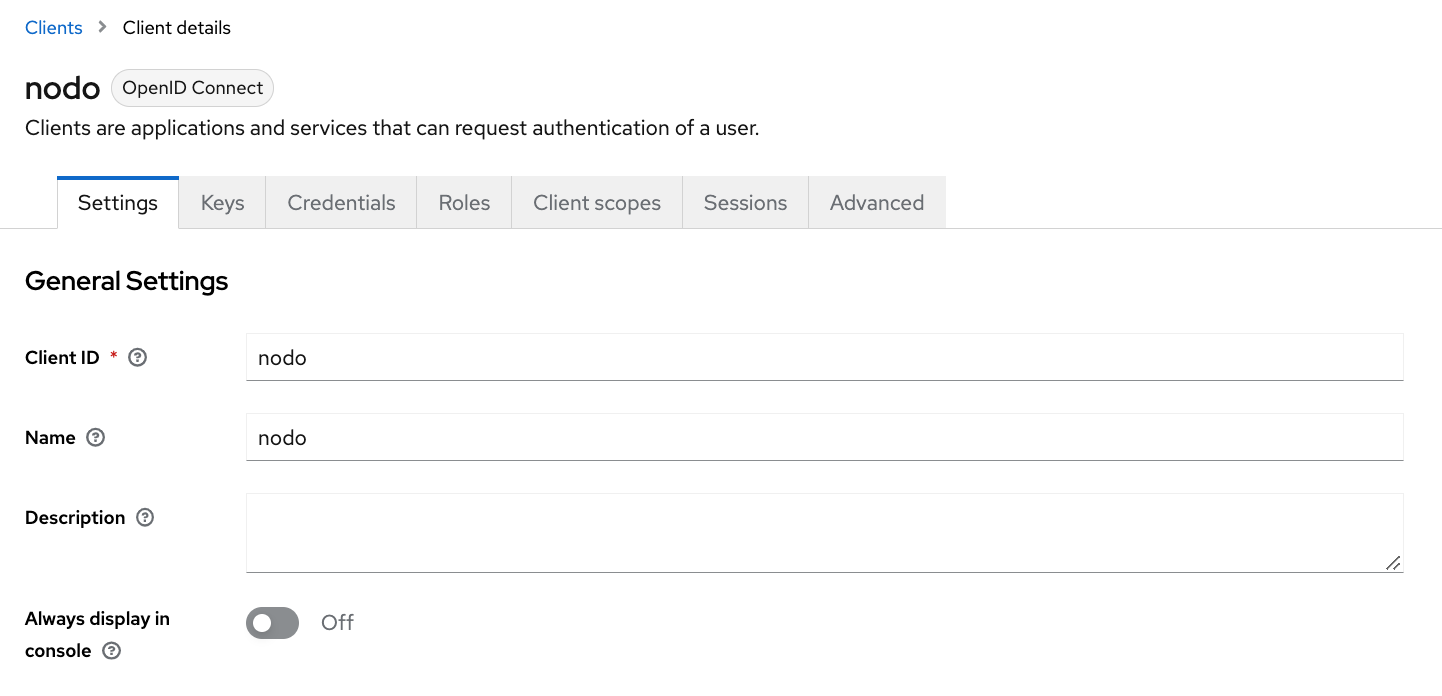
\includegraphics[width=0.9\linewidth]{Graphics/client_nodo}
	\caption{Cliente nodo}
	\label{fig:clientnodo}
\end{figure}

\begin{figure}[H]
	\centering
	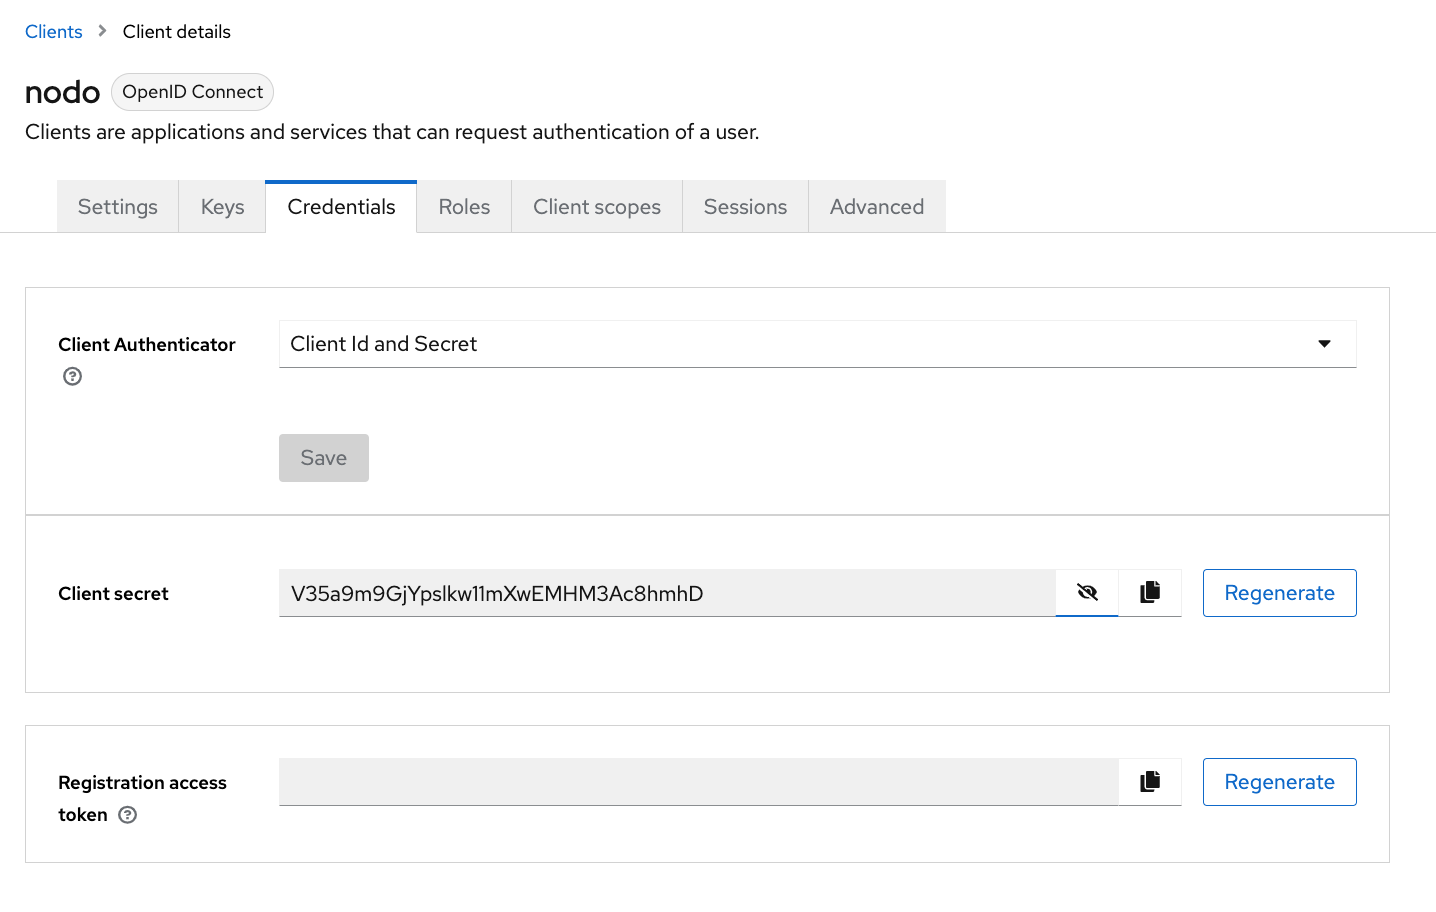
\includegraphics[width=0.9\linewidth]{Graphics/client_nodo_credentials}
	\caption{Credenciales del cliente nodo}
	\label{fig:clientnodocredentials}
\end{figure}

%\textcolor{red} {cómo se configura un cliente en keycloak?
%Qué endpoints expone la API de keycloak?
%Hablar sobre la biblioteca de python
%Poner el ejemplo de cómo se autentica}

\subsection*{Creación de cliente Keycloak para obtención de token}

En el siguiente código se muestra cómo se puede conectar el cliente a Keycloak a través de la biblioteca \textbf{python-keycloak}. También se crea una interfaz básica con Flask para visualizar los resultados.


\lstset{language=Python}
\lstset{frame=lines}
\lstset{caption={Conexión de cliente a Keycloak}}
\lstset{label={lst:code_direct}}
\lstset{basicstyle=\footnotesize}
\begin{lstlisting}
from flask import Flask
from flask import Flask, render_template, request
from keycloak.keycloak_openid import KeycloakOpenID
from keycloak.exceptions import KeycloakAuthenticationError, KeycloakGetError

import json

app = Flask(__name__)

keycloak_open_id = KeycloakOpenID(server_url="http://localhost:8080/", 
	client_id="nodo", 
	realm_name="master", 
	client_secret_key="secret key")
keycloak_open_id.well_know()

@app.route('/login', methods=['POST', 'GET'])
def login():
	error = None
	if request.method == 'POST':
		username = request.form['username']
		success, result = valid_login(username, request.form['password'])
		if success:
			return log_the_user_in(username, result["access_token"], result["refresh_token"])
		else:
			error = result["error_description"]
	# The code below is executed if the request method
	# was GET or the credentials were invalid
	return render_template('login.html', error=error)

def valid_login(username, password):
	# import pdb
	# pdb.set_trace()
	try:
		token = keycloak_open_id.token(username, password)
	except (KeycloakAuthenticationError, KeycloakGetError) as e:
		return False, json.loads(e.error_message)
	return True, token

def log_the_user_in(username, token, refresh_token):
	return render_template('success.html', username=username, token=token, refresh_token=refresh_token)
\end{lstlisting}


